%%%%%%%%%%%%%%%%%%%%%%%%%%%%%%%%%%%%%%%%%%%%%%%%%%%%%%%%%%
\begin{frame}
  \begin{beamerboxesrounded}{}
	\begin{center}

\vspace{20pt}

		MapReduce Integration

\vspace{20pt}

	\end{center}    
  \end{beamerboxesrounded}
\end{frame}


%%%%%%%%%%%%%%%%%%%%%%%%%%%%%%%%%%%%%%%%%%%%%%%%%%%%%%%%%%
\subsection{Recap}
%%%%%%%%%%%%%%%%%%%%%%%%%%%%%%%%%%%%%%%%%%%%%%%%%%%%%%%%%%
\frame {\frametitle{Introduction}
  \begin{itemize}
  \item \textbf{In the following we review the main classes involved in
      reading and writing data from/to an underlying data store}

    \vspace{20pt}

  \item \textbf{For MapReduce to work with HBase, some more practical issues
      have to be addressed}
    \begin{itemize}
    \item E.g.: creating an appropriate JAR file inclusive of all
      required libraries
    \end{itemize}

    \vspace{20pt}

  \item Refer to \cite{George2011}, Chapter 7 for an in-depth
    treatment of this subject
  \end{itemize}

}

\frame {\frametitle{Main classes involved in MapReduce}
  \begin{figure}[h]
    \centering
    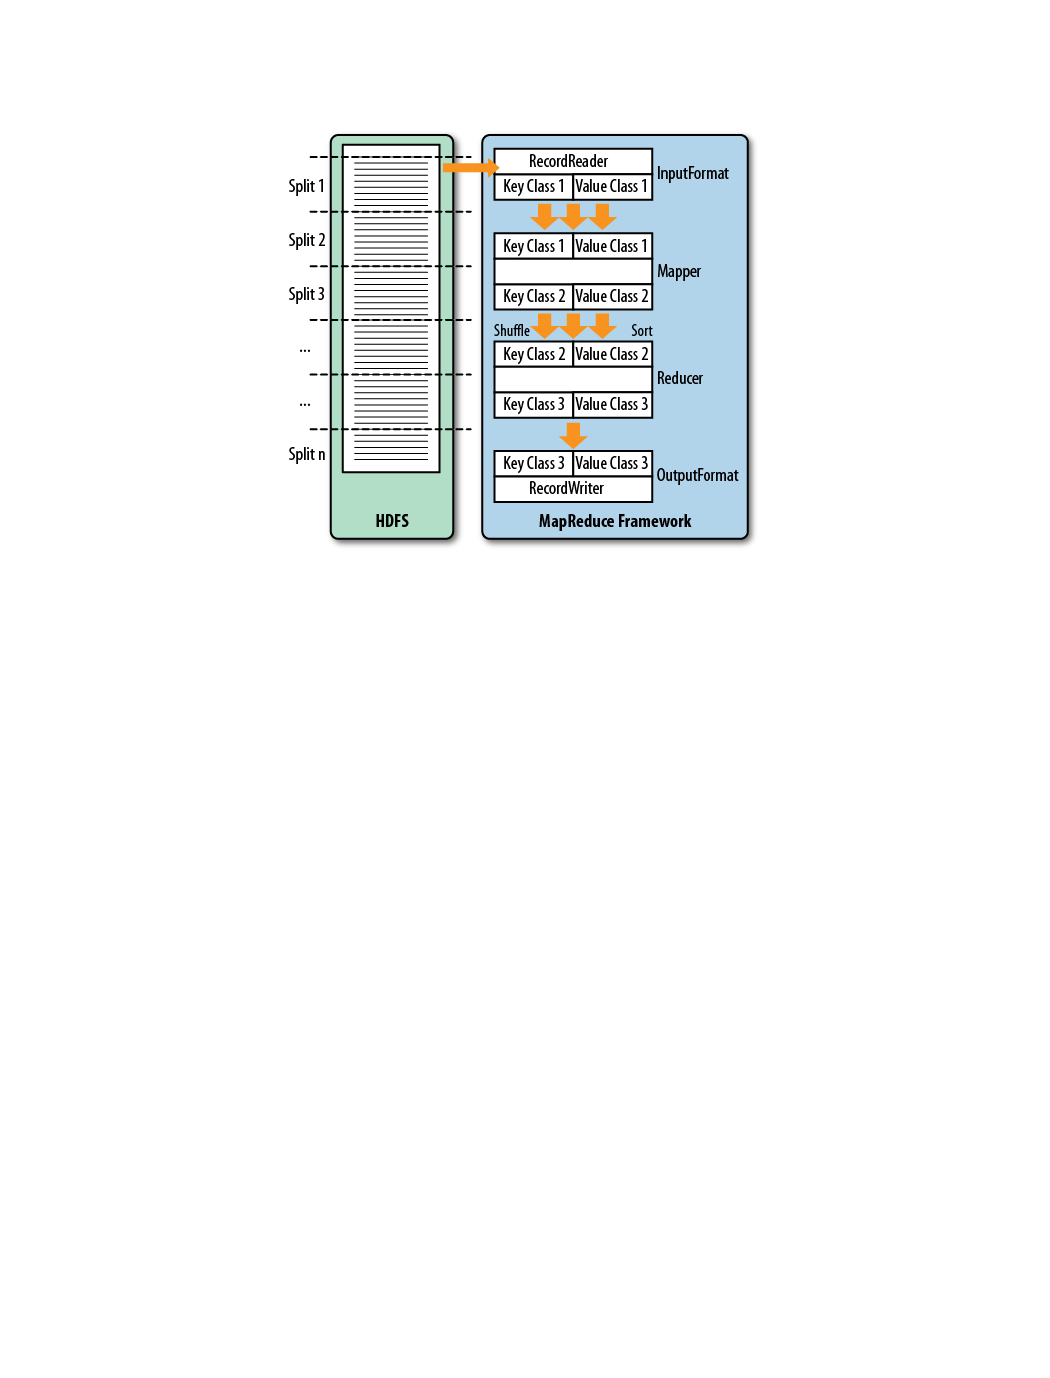
\includegraphics[scale=0.9]{./figures/mr-classes}
    \caption{Main MapReduce Classes}
  \end{figure}
}

\frame {\frametitle{Main classes involved in MapReduce}
  \begin{beamerboxesrounded}{}
    \texttt{InputFormat}
  \end{beamerboxesrounded}

  \begin{itemize}
  \item \textbf{It is responsible for two things}
    \begin{itemize}
    \item Splits input data
    \item Returns a \texttt{RecordReader} instance
      \begin{itemize}
      \item Defines a \textit{key} and a \textit{value} object
      \item Provides a \texttt{next()} method to iterate over input records
      \end{itemize}
    \end{itemize}
  \end{itemize}

  \begin{figure}[h]
    \centering
    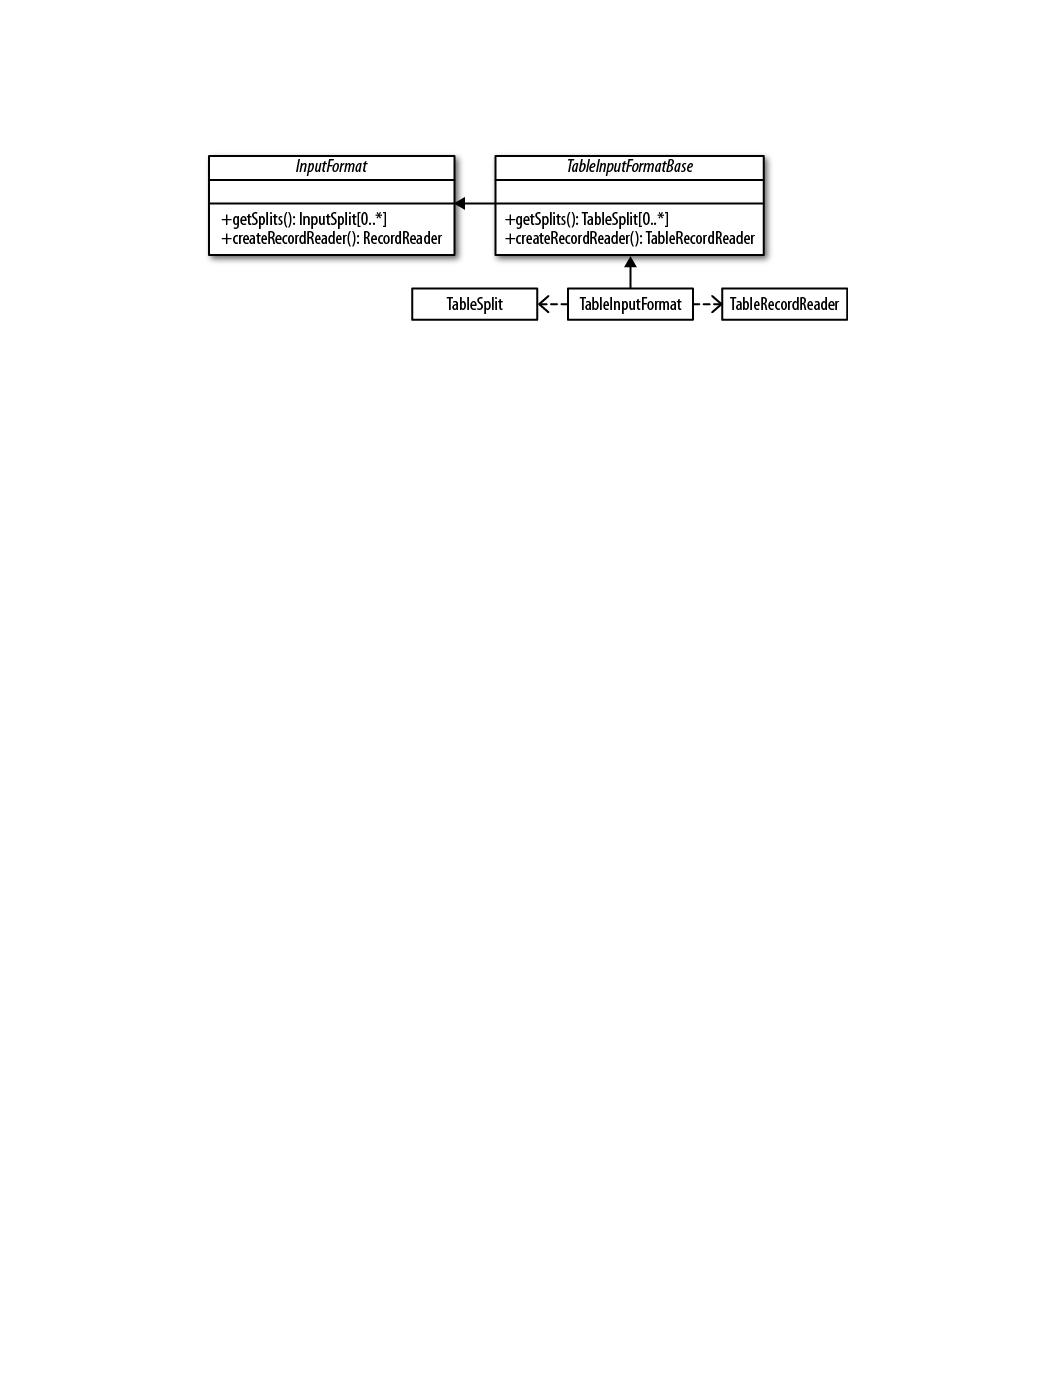
\includegraphics[scale=0.9]{./figures/input-format}
    \caption{InputFormat hierarchy}
    \label{fig:input-format}
  \end{figure}
}

\frame {\frametitle{Main classes involved in MapReduce}
  \begin{beamerboxesrounded}{}
    \texttt{InputFormat $\to$ TableInputFormatBase}
  \end{beamerboxesrounded}

  \begin{itemize}
  \item \textbf{Implement a full turnkey solution to scan an HBase
      table}
    \begin{itemize}
    \item Splits the table into proper blocks and hand them to the
      MapReduce process
    \end{itemize}

\vspace{20pt}

  \item \textbf{Must supply a \texttt{Scan} instance to interact with
      a table}
    \begin{itemize}
    \item Specify start and stop keys for the scan
    \item Add filters (optional)
    \item Specify the number of versions
    \end{itemize}
  \end{itemize}
}

\frame {\frametitle{Main classes involved in MapReduce}
  \begin{beamerboxesrounded}{}
    \texttt{Mapper}
  \end{beamerboxesrounded}

  \begin{itemize}
  \item \textbf{Each record read using the \texttt{RecordReader} is processed
    using the \texttt{map()} method}

  \vspace{20pt}

  \item \textbf{The \texttt{Mapper} reads specific types of input key/value
    pairs, but emit possibly another type}
  \end{itemize}

  \begin{figure}[h]
    \centering
    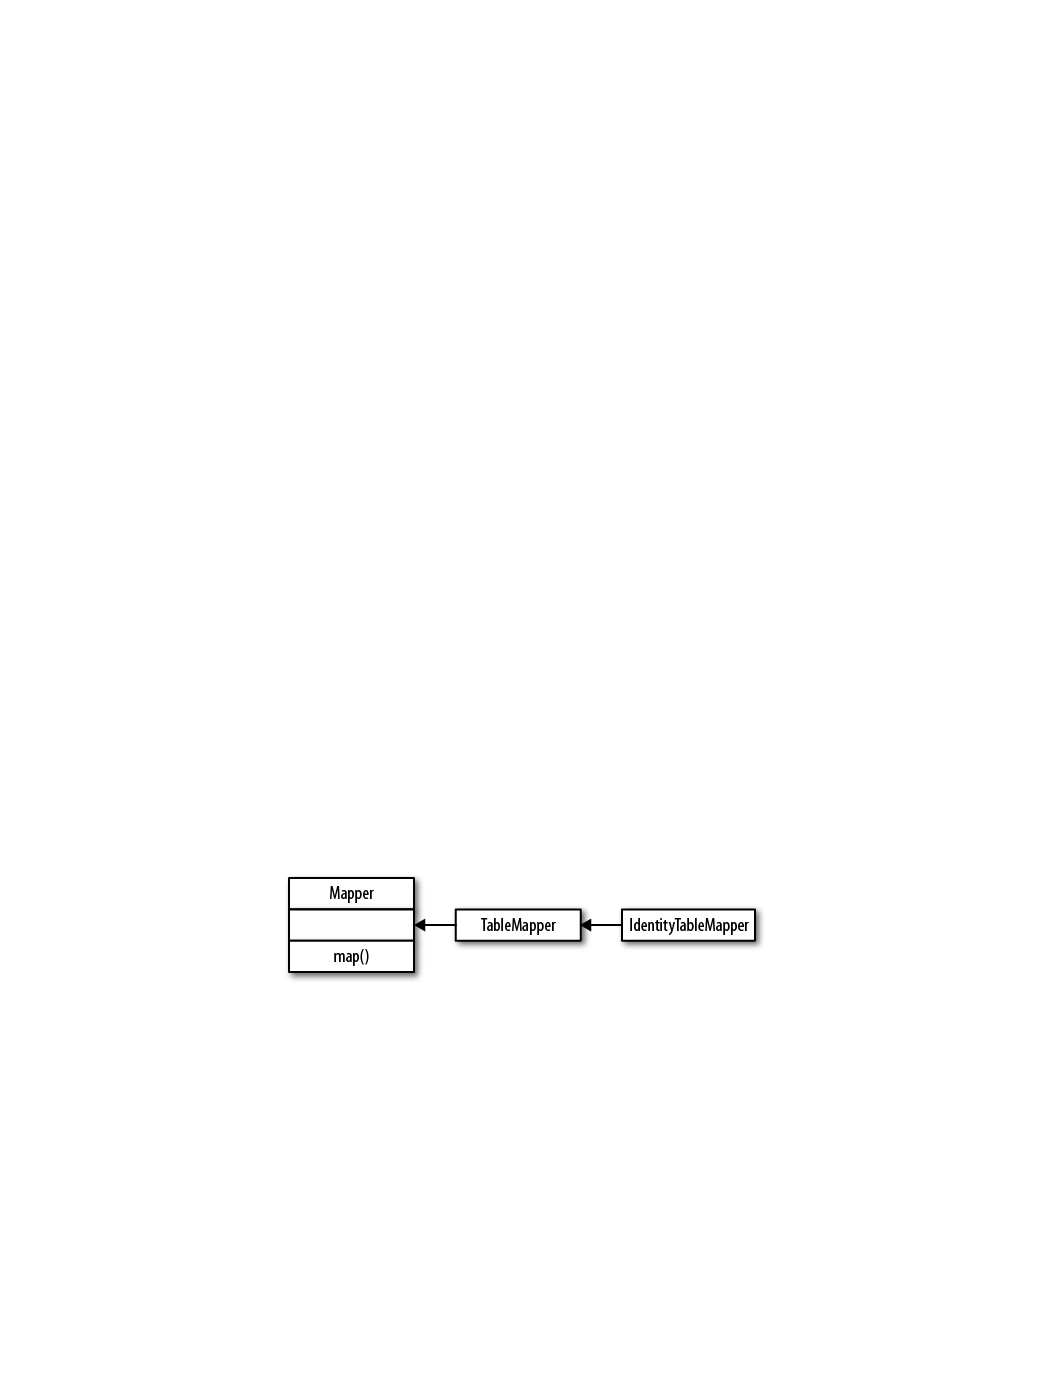
\includegraphics[scale=0.8]{./figures/mapper}
    \caption{The Mapper hierarchy}
    \label{fig:mapper}
  \end{figure}
}

\frame {\frametitle{Main classes involved in MapReduce}
  \begin{beamerboxesrounded}{}
    \texttt{Mapper $\to$ TableMapper}
  \end{beamerboxesrounded}

  \begin{itemize}
  \item \textbf{\texttt{TableMapper} class enforces:}
    \begin{itemize}
    \item The input key to the mapper to be an
      \texttt{ImmutableBytesWritable} type
    \item The input value to be a \texttt{Result} type
    \end{itemize}

    \vspace{20pt}

  \item \textbf{A handy implementation is the
      \texttt{IdentityTableMapper}}
    \begin{itemize}
    \item This is the equivalent of an identity mapper
    \end{itemize}
  \end{itemize}
}

\frame {\frametitle{Main classes involved in MapReduce}
  \begin{beamerboxesrounded}{}
    \texttt{OutputFormat}
  \end{beamerboxesrounded}

  \begin{itemize}
  \item \textbf{Used to persist data}
    \begin{itemize}
    \item Output written to files
    \item Output written to HBase tables
      \begin{itemize}
      \item This is done using a \texttt{TableRecordWriter}
      \end{itemize}
    \end{itemize}
  \end{itemize}

  \begin{figure}[h]
    \centering
    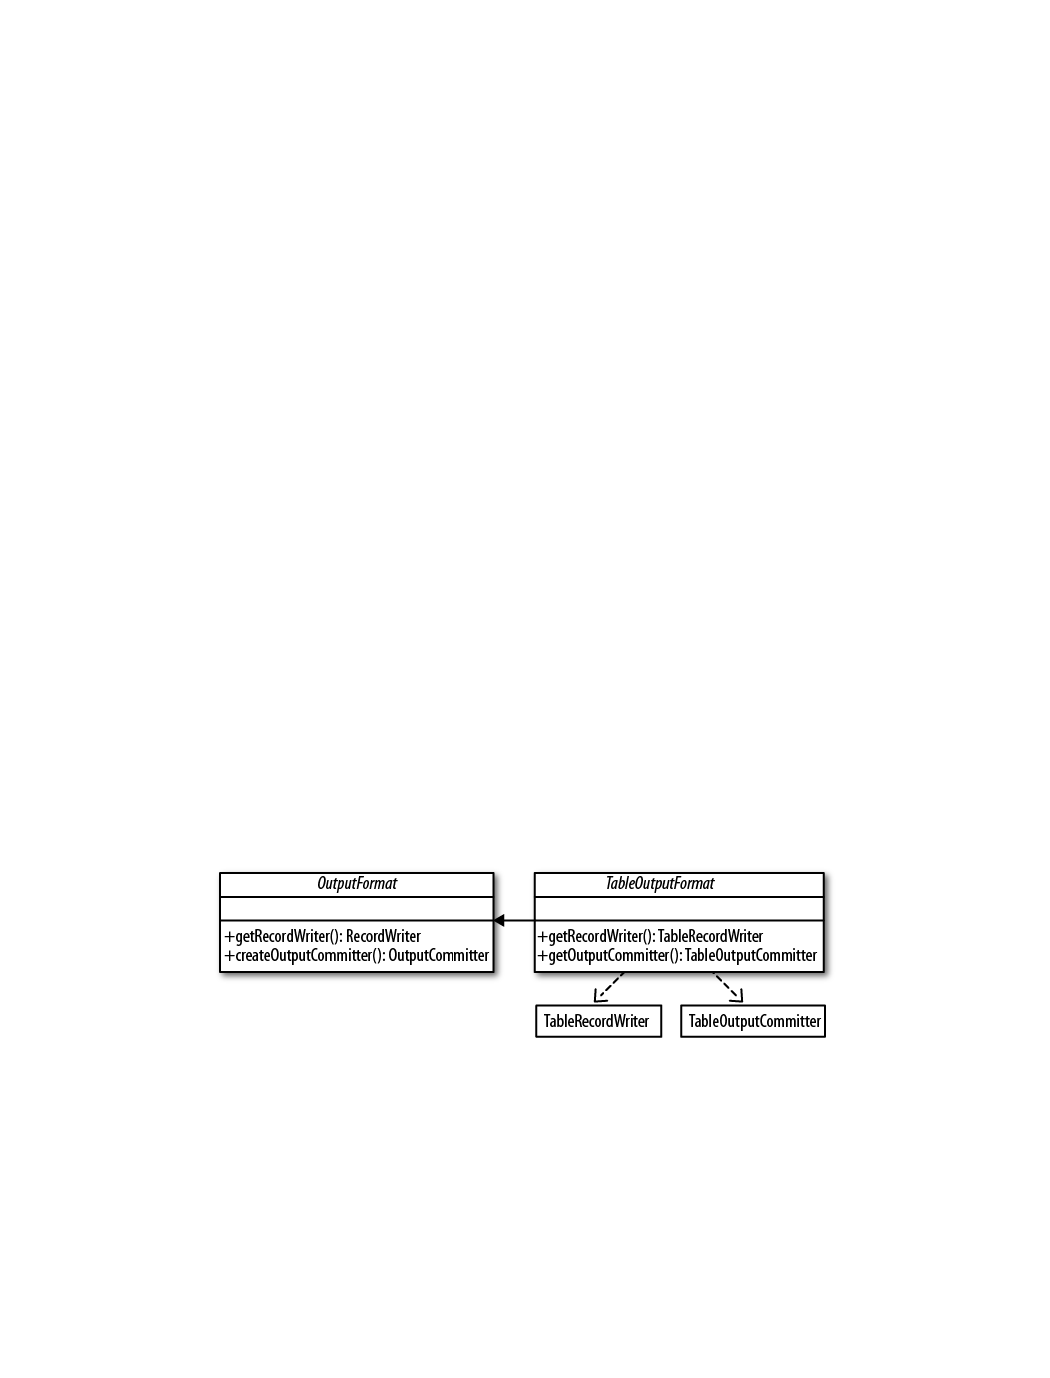
\includegraphics[scale=0.8]{./figures/outputformat}
    \caption{The OutputFormat hierarchy}
    \label{fig:outputformat}
  \end{figure}
}

\frame {\frametitle{Main classes involved in MapReduce}
  \begin{beamerboxesrounded}{}
    \texttt{OutputFormat $\to$ TableOutputFormat}
  \end{beamerboxesrounded}

  \begin{itemize}
  \item \textbf{This is the class that handles the key/valu pairs and writes
      them to their final destination}
    \begin{itemize}
    \item Single instance that takes the output record from each reducer subsequently
    \end{itemize}

    \vspace{20pt}

  \item \textbf{Details}
    \begin{itemize}
    \item Must specify the table name when the MR job is created
    \item Handles buffer flushing implicitly (\textit{autoflush} option is set to false)
    \end{itemize}
  \end{itemize}
}

\frame {\frametitle{MapReduce Locality}
  \begin{itemize}
  \item \textbf{How does the system make sure data is placed close to where it
      is needed?}
    \begin{itemize}
    \item This is done implicitly by MapReduce when using HDFS
    \item When MapReduce uses HBase things are a bit different
    \end{itemize}
    
    \vspace{20pt}
    
  \item \textbf{How HBase handles data locality}
    \begin{itemize}
    \item Shared vs. non-shared cluster
    \item HBase store its files on HDFS (\texttt{HFiles} and WAL)
    \item HBase servers are not restarted frequently and they perform
      compactions regularly
    \item[$\to$] HDFS is smart enough to ensure data locality
      \begin{itemize}
      \item There is a block placement policy that enforces local
        writes 
      \item The data node compares the server name of the writer with
        its own
      \item If they match, the block is written to the local filesystem
      \end{itemize}
    \item Just be careful about region movements during load balancing
      or server failures
    \end{itemize}

  \end{itemize}
}

\frame {\frametitle{Table Splits}
  \begin{itemize}
  \item \textbf{When running a MapReduce job that reads from an HBase table
      you use the \texttt{TableInputFormat}}
    \begin{itemize}
    \item Overrides \texttt{getSplits()} and \texttt{createRecordReader()}
    \end{itemize}

    \vspace{20pt}

  \item \textbf{Before a job is run, the framework calls getSplit() to
      determine how the data is to be separated into chunks}
    \begin{itemize}
    \item \texttt{TableInputFormat}, given the \texttt{Scan} instance
      you define, divide the table at region boundaries
    \item[$\to$] The number of input splits is equal to all regions
      between the start and stop keys
    \end{itemize}
  \end{itemize}
}


\frame {\frametitle{Table Splits}
  \begin{itemize}
  \item \textbf{When a job starts, the framework calls
      \texttt{createRecordReader()} for each input split}
    \begin{itemize}
    \item It iterates over the splits and create a new
      \texttt{TableRecordReader} with the current split
    \item Each \texttt{TableRecordReader} handles exactly one region,
      reading and mapping every row from the region's start and end keys
    \end{itemize}

    \vspace{20pt}

  \item \textbf{Data locality}
    \begin{itemize}
    \item Each split contains the server name hosting the region
    \item The framework checks the server name and if the
      \texttt{TaskTracker} is running on the same machine, it will run
      it on that server
    \item The \texttt{RegionServer} is colocated with the HDFS
      \texttt{DataNode}, hence data is read from the local filesystem
    \end{itemize}


    \vspace{20pt}

  \item \textbf{TIP: Turn off speculative execution!}


  \end{itemize}
}